\begin{figure}[H]
    \centering
    \definecolor{planetblue}{RGB}{75,145,205}
    \definecolor{radiusred}{RGB}{185,45,45}
    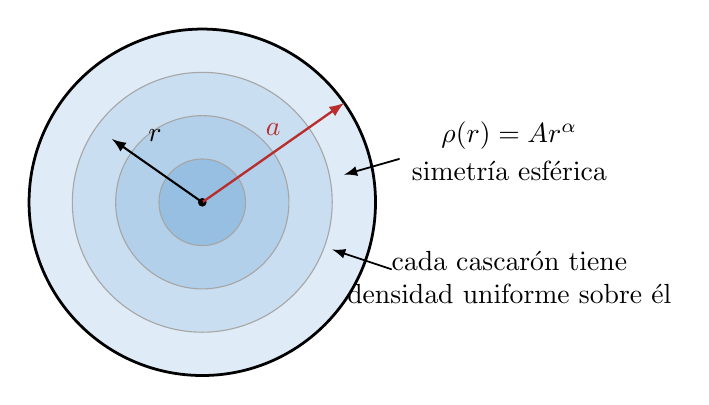
\begin{tikzpicture}[x=1cm,y=1cm,line cap=round,line join=round]
        \coordinate (O) at (4.15,2.50);

        % Capas esféricas representativas
        \fill[planetblue!18] (O) circle (2.20);
        \fill[planetblue!30] (O) circle (1.65);
        \fill[planetblue!43] (O) circle (1.10);
        \fill[planetblue!58] (O) circle (0.55);
        \draw[line width=1.0pt] (O) circle (2.20);
        \draw[black!35] (O) circle (1.65);
        \draw[black!35] (O) circle (1.10);
        \draw[black!35] (O) circle (0.55);
        \fill (O) circle (0.055);

        % Coordenadas radiales
        \draw[radiusred,-latex,line width=0.85pt]
            (O) -- ++(35:2.20);
        \node[radiusred,above] at (5.05,3.22) {$a$};
        \draw[-latex,line width=0.75pt]
            (O) -- ++(145:1.40);
        \node[above] at (3.55,3.15) {$r$};

        \node[align=center] at (8.05,3.15)
            {$\rho(r)=A r^\alpha$\\[2pt]
             simetría esférica};
        \draw[-latex,line width=0.65pt]
            (6.65,3.05) -- (5.95,2.85);

        \node[align=center] at (8.05,1.55)
            {cada cascarón tiene\\densidad uniforme sobre él};
        \draw[-latex,line width=0.65pt]
            (6.55,1.65) -- (5.80,1.90);
    \end{tikzpicture}
    \caption{Planeta esférico con densidad radial $\rho(r)=A r^\alpha$ y radio exterior $a$.}
\end{figure}
